\documentclass[10pt]{article}
\usepackage{tikz}
\usetikzlibrary{shapes.misc}
\usepackage[margin=0cm]{geometry}
\pagestyle{empty}
\tikzstyle{every node}=[cross out, draw, red]

\begin{document}

\vspace*{\fill}
\begin{center}
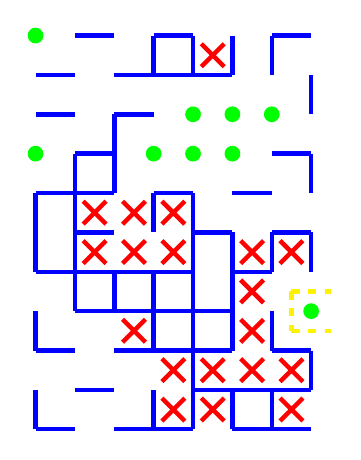
\begin{tikzpicture}[x=0.5cm, y=-0.5cm, ultra thick, blue]
% Walls
    \draw (1,0) -- (2,0);
    \draw (3,0) -- (4,0);
    \draw (6,0) -- (7,0);
    \draw (0,1) -- (1,1);
    \draw (2,1) -- (5,1);
    \draw (0,2) -- (1,2);
    \draw (2,2) -- (3,2);
    \draw (1,3) -- (2,3);
    \draw (6,3) -- (7,3);
    \draw (0,4) -- (2,4);
    \draw (3,4) -- (4,4);
    \draw (5,4) -- (6,4);
    \draw (1,5) -- (2,5);
    \draw (4,5) -- (5,5);
    \draw (6,5) -- (7,5);
    \draw (0,6) -- (4,6);
    \draw (5,6) -- (6,6);
    \draw (1,7) -- (5,7);
    \draw (0,8) -- (1,8);
    \draw (2,8) -- (5,8);
    \draw (6,8) -- (7,8);
    \draw (1,9) -- (2,9);
    \draw (4,9) -- (7,9);
    \draw (0,10) -- (1,10);
    \draw (2,10) -- (4,10);
    \draw (5,10) -- (7,10);
    \draw (0,4) -- (0,6);
    \draw (0,7) -- (0,8);
    \draw (0,9) -- (0,10);
    \draw (1,3) -- (1,7);
    \draw (2,2) -- (2,4);
    \draw (2,6) -- (2,7);
    \draw (3,0) -- (3,1);
    \draw (3,4) -- (3,5);
    \draw (3,6) -- (3,8);
    \draw (3,9) -- (3,10);
    \draw (4,0) -- (4,1);
    \draw (4,4) -- (4,10);
    \draw (5,0) -- (5,1);
    \draw (5,5) -- (5,8);
    \draw (5,9) -- (5,10);
    \draw (6,0) -- (6,1);
    \draw (6,5) -- (6,6);
    \draw (6,7) -- (6,8);
    \draw (6,9) -- (6,10);
    \draw (7,1) -- (7,2);
    \draw (7,3) -- (7,4);
    \draw (7,5) -- (7,6);
    \draw (7,8) -- (7,9);
% Pillars
    \fill[green] (0,0) circle(0.2);
    \fill[green] (4,2) circle(0.2);
    \fill[green] (5,2) circle(0.2);
    \fill[green] (6,2) circle(0.2);
    \fill[green] (0,3) circle(0.2);
    \fill[green] (3,3) circle(0.2);
    \fill[green] (4,3) circle(0.2);
    \fill[green] (5,3) circle(0.2);
    \fill[green] (7,7) circle(0.2);
% Inner points in accessible cul-de-sacs
    \node at (4.5,0.5) {};
    \node at (1.5,4.5) {};
    \node at (2.5,4.5) {};
    \node at (3.5,4.5) {};
    \node at (1.5,5.5) {};
    \node at (2.5,5.5) {};
    \node at (3.5,5.5) {};
    \node at (5.5,5.5) {};
    \node at (6.5,5.5) {};
    \node at (5.5,6.5) {};
    \node at (2.5,7.5) {};
    \node at (5.5,7.5) {};
    \node at (3.5,8.5) {};
    \node at (4.5,8.5) {};
    \node at (5.5,8.5) {};
    \node at (6.5,8.5) {};
    \node at (3.5,9.5) {};
    \node at (4.5,9.5) {};
    \node at (6.5,9.5) {};
% Entry-exit paths without intersections
    \draw[dashed, yellow] (6.5,6.5) -- (7.5,6.5);
    \draw[dashed, yellow] (6.5,7.5) -- (7.5,7.5);
    \draw[dashed, yellow] (6.5,6.5) -- (6.5,7.5);
\end{tikzpicture}
\end{center}
\vspace*{\fill}

\end{document}
